\documentclass[11pt]{extarticle}
\usepackage[margin=25pt]{geometry}
\usepackage{babel}
\usepackage[T1]{fontenc}

\usepackage{fancyvrb}
\usepackage{adjustbox}
\usepackage{multicol}
\usepackage{graphicx}
\usepackage{tikz}
\usetikzlibrary{trees, calc, positioning}

\graphicspath{ {../assets/} }

\makeatletter
\def\app@exe{\immediate\write18}
\newread\tmpFile
\def\images#1{%
	\def\tmpFilePath{tmp/#1_\jobname.tmp}
	\def\imageDir{images/#1}
	\app@exe{ls -1 \imageDir > \tmpFilePath}
	\openin\tmpFile=\tmpFilePath
	\def\imageName{\imageDir/\image}
	\endlinechar=-1
	\read\tmpFile to \image
	\loop\unless\ifeof\tmpFile
		\def\imageName{\detokenize\expandafter{\image}}
		\begin{minipage}{0.2\textwidth}
			\centering
			\includegraphics[width=\textwidth]{\imageDir/\imageName}
		\end{minipage}
		\read\tmpFile to \image
	\repeat
	\closein\tmpFile
	\app@exe{rm \tmpFilePath}
	\\[2em]
}
\makeatother

\title{%
	{\Huge Elektronický herbár}
	\footnote{náhodných rastlín okolo školy :)}
}
\author{Adam Labuš, Sexta B}

\def\ruler{%
	\vspace{0.5em}
	\noindent\rule{\textwidth}{0.5pt}
	\vspace{0.5em}
}

\begin{document}
	\maketitle

	\section{Úvod}
	\subsection{Informácie k fotografiám}
	\begin{center}
		\begin{tabular}{ |c|c|c| }
		\hline
		Miesto zberu & okolie školy \\
		Fotograf & Richard Letaši \\
		Rastliny určil & Adam Labuš \\
		Dátum zberu & 12.4.2024 \\
		\hline
		\end{tabular}
	\end{center}

	\newpage
	\subsection{Zaradenie}
	\begin{center}
		\large
		\begin{adjustbox}{max width=.9\paperheight, angle=90}
		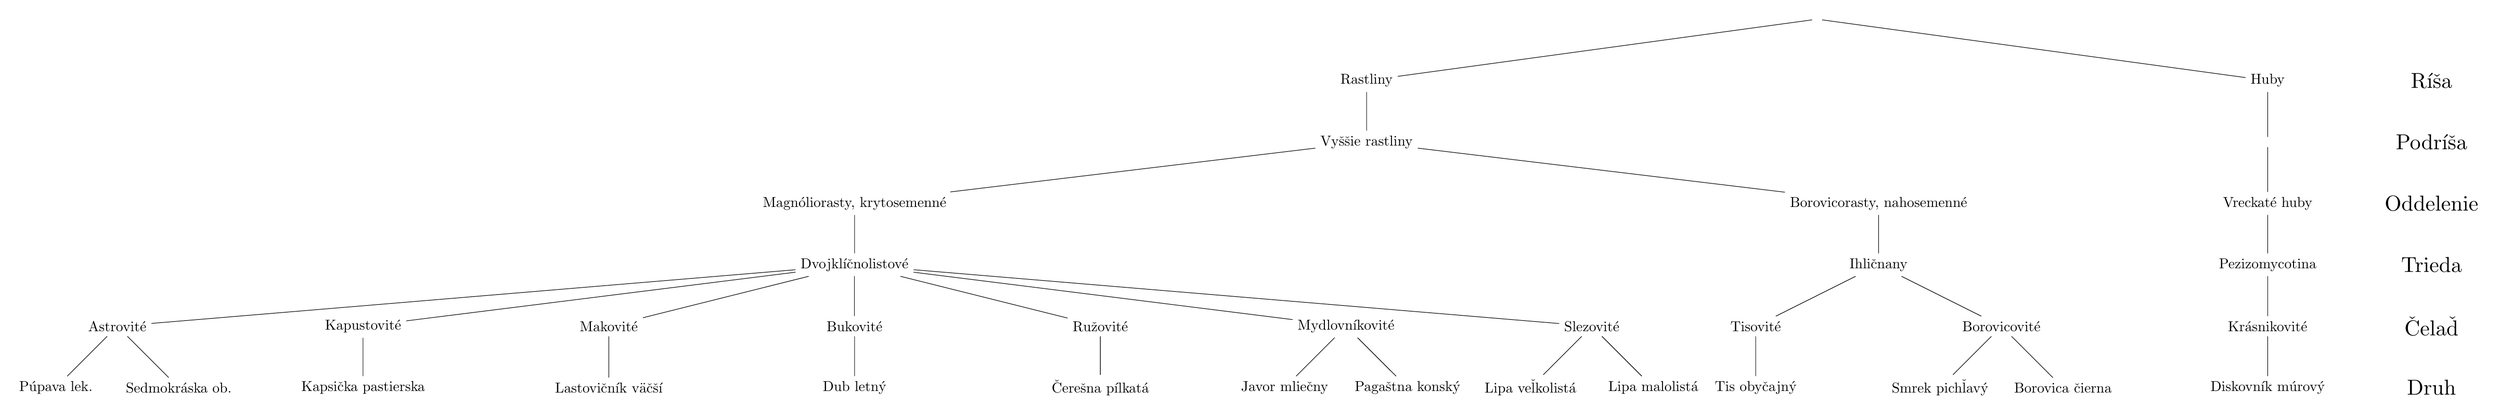
\begin{tikzpicture}[
			level distance=1.5cm,
	 		level 1/.style={sibling distance=22cm},
	 		level 2/.style={sibling distance=15cm},
	 		level 3/.style={sibling distance=25cm},
	 		level 4/.style={sibling distance=15cm},
	 		level 5/.style={sibling distance=15cm},
	 		level 5/.style={sibling distance=6cm},
	 		level 6/.style={sibling distance=3cm},
			layer/.style={scale=1.5}
		]
			\node {}
				child { node {Rastliny}
					child { node {Vyššie rastliny}
						child { node {Magnóliorasty, krytosemenné}
							child { node {Dvojklíčnolistové}
								child { node {Astrovité}
									child { node {Púpava lek.} }
									child { node {Sedmokráska ob.} }
								}
								child { node {Kapustovité}
									child { node {Kapsička pastierska} }
								}
								child { node {Makovité}
									child { node {Lastovičník väčší}}
								}
								child { node {Bukovité}
									child { node {Dub letný}}
								}
								child { node {Ružovité}
									child { node {Čerešna pílkatá}}
								}
								child { node {Mydlovníkovité}
									child { node {Javor mliečny}}
									child { node {Pagaštna konský}}
								}
								child { node {Slezovité}
									child { node {Lipa veľkolistá}}
									child { node {Lipa malolistá}}
								}
							}
						}
						child { node {Borovicorasty, nahosemenné}
							child { node {Ihličnany}
								child { node {Tisovité}
									child { node {Tis obyčajný} }
								}
								child { node {Borovicovité}
									child { node {Smrek pichľavý} }
									child { node {Borovica čierna} }
								}
							}
						}
					}
				}
				child { node {Huby}
					child { node {}
						child { node {Vreckaté huby}
							child { node {Pezizomycotina}
								child { node {Krásnikovité}
									child { node {Diskovník múrový}}
								}
							}
						}
					}
				};

			\node[layer] at (15,-1.5) {Ríša};
			\node[layer] at (15,-3) {Podríša};
			\node[layer] at (15,-4.5) {Oddelenie};
			\node[layer] at (15,-6) {Trieda};
			\node[layer] at (15,-7.5) {Čelaď};
			\node[layer] at (15,-9) {Druh};
		\end{tikzpicture}
		\end{adjustbox}
	\end{center}
	\newpage
	\tableofcontents
	\newpage

	\section{Stromy}
	\subsection{Smrek pichľavý - Picea pungens}
	\images{smrek}
	\ruler

	\subsection{Lipa malolistá - Tilia cordata}
	\images{lipa_malolista}
	\ruler

	\subsection{Javor mliečny - Acer platanoides}
	\images{javor_horsky}
	\ruler

	\subsection{Borovica čierna - Pinus nigra}
	\images{borovica}
	\ruler

	\subsection{Čerešňa pilkatá - Prunus serrulata}
	\images{ceresna}
	\ruler

	\subsection{Dub letný - Quercus robur}
	\images{dub}
	\ruler

	\subsection{Pagaštan konský - Aesculus hippocastanum}
	\images{pagastan_konsky}
	\ruler

	\subsection{Lipa veľkolistá - Tilia platyphyllos}
	\images{lipa_velkolista}
	\ruler

	\section{Kry}

	\subsection{Tis obyčajný - Taxus baccata}
	\images{tis}
	\ruler

	\subsection{Kaliná vráskavolistá}
	\images{kalina}
	\ruler

	\section{Kvety}

	\subsection{Lastovničník väčší - Chelidonium majus}
	\images{lastovicnik_vacsi}
	\ruler

	\subsection{Sedmokráska obyčajná - Bellis perennis}
	\images{sedmokraska}
	\ruler

	\subsection{Púpava lekárska - Taraxacum officinale}
	\images{pupava}
	\ruler

	\subsection{Kapsička pastierska - Capsella bursa-pastoris}
	\images{kapsicka_pastierska}
	\ruler
	
	\section{Machorasty}
	\subsection{}
	\images{mach}
	\ruler

	\section{Lišajníky}
	
	\subsection{Diskovník múrový - Xanthoria parietina}
	\images{lisajnik}
	\ruler
\end{document}
